\renewcommand{\one}{fake_030}
\renewcommand{\two}{real_other-bamboo-veawe}

\setlength{\resLen}{0.556in}
\begin{figure*}[tbhp]
	\addtolength{\tabcolsep}{-4pt}
	\begin{tabular}{lcccc@{\hspace{2\tabcolsep}}ccc}
		& & \textbf{\small SVBRDF maps} &
		\multicolumn{2}{c}{\textbf{\small Novel views}}
		& \textbf{\small SVBRDF maps} & 
		\multicolumn{2}{c}{\textbf{\small Novel views}}
		\\
		& \raisebox{.25in}{\rotatebox[origin=c]{90}{\footnotesize{GT}}} &
		\includegraphics[height=\resLen]{results/init/\one/ref/tex.jpg} &
		\includegraphics[height=\resLen]{results/init/\one/ref/07.jpg} &
		\includegraphics[height=\resLen]{results/init/\one/ref/08.jpg} &
		 &
		\includegraphics[height=\resLen]{results/init/\two/ref/07.jpg} &
		\includegraphics[height=\resLen]{results/init/\two/ref/08.jpg}
		\\
		& \raisebox{.25in}{\rotatebox[origin=c]{90}{\footnotesize{[Deschaintre]}}} &
		\includegraphics[height=\resLen]{results/init/\one/egsr/tex.jpg} &
		\includegraphics[height=\resLen]{results/init/\one/egsr/07.jpg} &
		\includegraphics[height=\resLen]{results/init/\one/egsr/08.jpg} &
		\includegraphics[height=\resLen]{results/init/\two/egsr/tex.jpg} &
		\includegraphics[height=\resLen]{results/init/\two/egsr/07.jpg} &
		\includegraphics[height=\resLen]{results/init/\two/egsr/08.jpg}
		\\
		\hline\\[-8pt]
		\multirow{2}{*}[1em]{\rotatebox[origin=c]{90}{\footnotesize\bfseries Constant init.}} &
		\raisebox{.25in}{\rotatebox[origin=c]{90}{\footnotesize{Ours}}} &
		\includegraphics[height=\resLen]{results/init/\one/ours+/tex.jpg} &
		\includegraphics[height=\resLen]{results/init/\one/ours+/07.jpg} &
		\includegraphics[height=\resLen]{results/init/\one/ours+/08.jpg} &
		\includegraphics[height=\resLen]{results/init/\two/ours+/tex.jpg} &
		\includegraphics[height=\resLen]{results/init/\two/ours+/07.jpg} &
		\includegraphics[height=\resLen]{results/init/\two/ours+/08.jpg}
		\\
		& \raisebox{.25in}{\rotatebox[origin=c]{90}{\footnotesize{[Gao19]}}} &
		\includegraphics[height=\resLen]{results/init/\one/msra+/tex.jpg} &
		\includegraphics[height=\resLen]{results/init/\one/msra+/07.jpg} &
		\includegraphics[height=\resLen]{results/init/\one/msra+/08.jpg} &
		\includegraphics[height=\resLen]{results/init/\two/msra+/tex.jpg} &
		\includegraphics[height=\resLen]{results/init/\two/msra+/07.jpg} &
		\includegraphics[height=\resLen]{results/init/\two/msra+/08.jpg}
		\\
		\hline\\[-8pt]
		\multirow{2}{*}[3.15em]{\rotatebox{90}{\footnotesize\bfseries [Deschaintre]-based init.}} &
		\raisebox{.25in}{\rotatebox[origin=c]{90}{\footnotesize{Ours+}}} &
		\includegraphics[height=\resLen]{results/init/\one/ours+_egsr/tex.jpg} &
		\includegraphics[height=\resLen]{results/init/\one/ours+_egsr/07.jpg} &
		\includegraphics[height=\resLen]{results/init/\one/ours+_egsr/08.jpg} &
		\includegraphics[height=\resLen]{results/init/\two/ours+_egsr/tex.jpg} &
		\includegraphics[height=\resLen]{results/init/\two/ours+_egsr/07.jpg} &
		\includegraphics[height=\resLen]{results/init/\two/ours+_egsr/08.jpg}
		\\
		& \raisebox{.25in}{\rotatebox[origin=c]{90}{\footnotesize{[Gao19]+}}} &
		\includegraphics[height=\resLen]{results/init/\one/msra+_egsr/tex.jpg} &
		\includegraphics[height=\resLen]{results/init/\one/msra+_egsr/07.jpg} &
		\includegraphics[height=\resLen]{results/init/\one/msra+_egsr/08.jpg} &
		\includegraphics[height=\resLen]{results/init/\two/msra+_egsr/tex.jpg} &
		\includegraphics[height=\resLen]{results/init/\two/msra+_egsr/07.jpg} &
		\includegraphics[height=\resLen]{results/init/\two/msra+_egsr/08.jpg}
		\\
	\end{tabular}
	\caption{\label{fig:result_init}
		\textbf{SVBRDF results with different initialization} Unlike Gao's method, ours is less strongly dependent on a good initialization from Deschaintre's method~\shortcite{Deschaintre2019}. In most of cases, starting from simple texture maps (given by our constant initializations) is already good enough to converge to a clean solution. We show all combinations (with and without good initializations) for both methods, for one synthetic and one real example, where techniques initialized with [Deschaintre] are denoted with the suffix ``+'' (i.e., ``Ours+'' and ``[Gao19]+''). Note the failure of Gao's method without good initializations (i.e., ``Gao19'').}
\end{figure*}

